\documentclass[12pt, a4paper, hidelinks]{article}

\usepackage{natbib}
\usepackage{codestyle}
\usepackage{graphicx}
\usepackage{hyperref}
\usepackage{makecell}
\usepackage{booktabs}
\usepackage{threeparttablex}
\usepackage[margin = 2cm]{geometry}

\usepackage{amsmath}
\usepackage{amssymb}

\title{Reproduction of Erin Hengel 2017}
\author{Chia-Wei, Chen \thanks{r10323045@ntu.edu.tw}}



\begin{document}

\maketitle

\tableofcontents

\section*{Introduction}
This project is to reproduce Erin Hengel (\citeyear{Hengel17}) on "Publishing While  Female". The main work is to get all articles with abstracts
\footnote{Some are not explicitly abstracts. See further chapter} 
from five well-known economics journals and match each articles with a gender score.

Therefore scaping articles and authors' genders are a crucial task of this job.
\newpage

\section{Current Progress}

I mainly finish the following tasks. 

\begin{enumerate}
    \item Scraping abstract from AER, ECA, JPE, QJE, and RES \footnote{These are respectively, \emph{The American Economic Review, Econometrica, Journal of Political Economy, Quarterly Journal of Economics}, and \emph{The Review of Economic Studies} }. 
    
    \item For articles in JPE, some abstracts are provided explicitly, not in html text form, but in the first-page image. I extracted them via image processing.
    
    \item Extracted Authors' genders from Erin Hengel's \href{https://www.erinhengel.com/data/articles/}{Website.}
    
    \item Construct a python file to convert all results into regression-ready format.
\end{enumerate}

I will then describe in detail what I have done and what I am not able to complete. Note that the work is somehow messy and might be hard to tract. I will do my best to guide you through my processes. 

% =================================
%
%
%
%        Scrpaing
%
%
%
%==================================

\subsection{Scraping}

Table \ref{tab:scrape_source} shows the source of abstract for each journal:

\begin{table}[h]
    \centering
    \begin{tabular}{c l l l }
        \toprule
    Journal & Years & Source & \thead{Scraped by \\ previous person}\\
        \midrule
        AER & After 1999 & AEA web & \checkmark \\
         & 1980 to 1999 & JSTOR & \\ 
        ECA & 1950 to 2022 & JSTOR & \\
        JPE & 1960 to 2022 & Chicago Press Journals&\\
        QJE & 1980 to 2022 & Oxford Academic & \checkmark\\
        REStud & 1980 to 2022 & Oxford Academic & \checkmark \\
        \bottomrule
    \end{tabular}
    \caption{Source and Years of scraping for each journal.}
    \label{tab:scrape_source}
\end{table}

Several results are already provided hence I worked on and scraped only AER, ECA, JPE. Technical details are provided in future chapters. I simply scraped the "Abstract" element on the \verb|html|. However, there are discrepancies with the results provided by \cite{Hengel17}, see figure \ref{fig:HengelNum}

\begin{figure}[h]
    \centering
    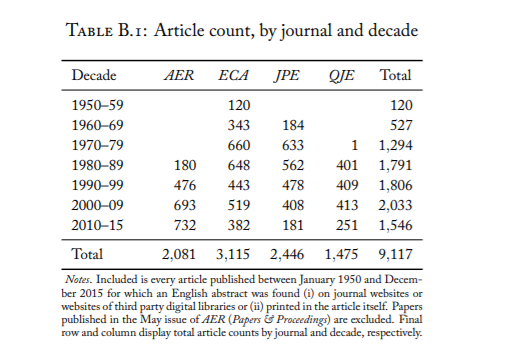
\includegraphics[width = 0.7\textwidth]{IMG/article count.png}
    \caption{Numbers of articles with abstract provided By Hengel}
    \label{fig:HengelNum}
\end{figure}

The result I scraped is shown in table \ref{tab:compare_scrape} in page \pageref{tab:compare_scrape}. Table \ref{tab:compare_scrape} shows several discrepancies that have to be checked manually, and I haven't tackle, and have no clue how, yet. 

\begin{table}[t]
    \centering
    \caption{Scraped and image processed result compared with \cite{Hengel17}}
    \label{tab:compare_scrape}
    \begin{threeparttable}
    \begin{tabular}{*4c}
        \toprule
        Decade & Scrape & Hengel & Note \\
        \midrule
        \multicolumn{4}{c}{AER} \\
        \midrule
        1980 - 1989  & 181 & 180 & \\
        1990 - 1999  & 512 & 476 & \\
        2000 - 2009  & 682 & 693 & \\
        2010 - 2015  & 733 & 732 & \\
        \midrule

        \multicolumn{4}{c}{ECA} \\
        \midrule
        1950 - 1959 & 130 & 120 & \makecell{Non-english \\ articles} \\
        1960 - 1969 & 344 & 343 & \\
        1970 - 1979 & 661 & 660 & \\
        1980 - 1989 & 648 & 648 & \\
        1990 - 1999 & 443 & 443 & \\
        2000 - 2009 & 520 & 520 & \\
        2010 - 2015 & 384 & 382 & \\
        
        \midrule

        \multicolumn{4}{c}{JPE} \\
        \midrule
        1960 - 1969 & 0 & 184 & No official abstract \\
        1970 - 1979 & 448 & 633 & OCR results added \\
        1980 - 1989 & 559 & 562 & OCR results added \\
        1990 - 1999 & 478 & 478 & \\
        2000 - 2009 & 408 & 408 & \\
        2010 - 2015 & 181 & 181 & \\

        \midrule

        \multicolumn{4}{c}{QJE} \\
        \midrule
        1980 - 1989 & 393 & 401 & \\
        1990 - 1999 & 409 & 409 & \\
        2000 - 2009 & 413 & 413 & \\
        2010 - 2015 & 251 & 251 & \\
        \bottomrule
    \end{tabular}
    \begin{tablenotes}
        \small
        \item[*] For non-english articles, I excluded them when counting, but the article is still included in the combined raw data.
    \end{tablenotes}
\end{threeparttable}
\end{table}
\subsubsection*{Non-technical Description of the Scraping Process}

For each journal, I do the scraping in two steps. 

\begin{enumerate}
    \item Extract the list of articles from each issues within the time period. Save all articles into a single file, named \verb|~_all_issue.csv|
    \item Scrape the abstracts according to the source url.
\end{enumerate}

This allows me to easily separate the process into several segments.\footnote{The website usually arranges its articles in the following hierarchy: 1. Issues within decades 2. Articles withing issues. 3. Abstract within the webpage for each articles. Therefore it is a good idea to first extract all articles and its urls from all issues, then scrape the articles from the list of urls.}

\subsubsection*{AER}

\begin{itemize}
    \item Articles after 1999 are already scraped when I started the project; the original result is in the following folder: \\

    \begin{center}
        \verb| Already Scraped/American Economic Review|
    \end{center}

    \item I scraped those before 1999 because it is not provided in the official website of AER. I accessed those from JSTOR, and saved my raw results in 

    \begin{center}
        \verb|AER/AER.csv|
    \end{center} 

    \item Following \cite{Hengel17}, articles in May and "Comments", "Reply" etc., are neglected, and were not scraped in the first place.
    
    \item Discrepancies are shown in table\ref{tab:compare_scrape}.
\end{itemize}

\subsubsection*{ECA}

\begin{itemize}
    \item Results are stored in 
    \begin{center}
        \verb|ECA\ECA.csv|
    \end{center}
    \item To speed up scraping, I loaded all articles in JSTOR but skipped the ones with \emph{Report of,Report on, Annual Reports,Criticism Invited}. I kept the orginal list of articles (before filtering) in 
    \begin{center}
        \verb|ECA\ECA_all_issue.csv|
    \end{center}
    and kept those I skipped in
    \begin{center}
        \verb|ECA\ECA_skipped.csv|
    \end{center}
    \item Ignore the other \verb|csv| files. Those are for temporary use.
    \item I scraped all of them from JSTOR.
    \item Some are not in English. The discrepancies reduces to one or two after the filtering.
    \item The non-English articles are still included in the \verb|combined/all_combined.csv|, but it is easy to filter out.
    \item Discrepancies are shown in table \ref{tab:compare_scrape}. Which does not differ much.
\end{itemize}

\subsubsection*{JPE}

\begin{itemize}
    \item Results with abstracts are stored in 
    \begin{center}
        \verb|JPE/JPE.csv|
    \end{center}

    \item Original list of all articles is saved in
    \begin{center}
        \verb|JPE/JPE_all_issue.csv|
    \end{center} 

    \item The source is Chicago Press Journal. Some articles have abstracts in the front-page image, but the text is not provided as web element that is available for copying. 
    \item I handle some articles during 1970 - 1989 by image processing, which automatically extracted the abstract block and save them to the result file. 
    \item Images and its result are stored in 
    \begin{center}
        \verb|JPE\first_pages|
    \end{center}

    \item It seems that Hengel did not only consider explicitly the abstract, but also some fist paragraphs of articles, when abstracts are not found. 
    \item Manual work must be done to match the results of Hengel.

\end{itemize}

\subsubsection*{QJE}

\begin{itemize}
    \item Already scraped by previous work.
    \item I cleaned the format to match those I scraped, making it easier to merge.
\end{itemize}

\subsubsection*{REStud}
\begin{itemize}
    \item Already scraped by previous work.
    \item \cite{Hengel17} didn't provide her results.
    \item I also cleaned the format.
\end{itemize}


% =================================
%
%
%
%        Gender
%
%
%
%==================================

\subsection{Gender}

Gender detail is extracted from Hengel's website. The original data can be found in 
\begin{center}
    \verb|Authors/.|
\end{center}

Each folder in the \verb|Authors/| directory is a list of readability scores of Economists, categorized by the first letter of its last name, as shown in figure \ref{fig:author_list}
\begin{figure}[h]
    \centering
    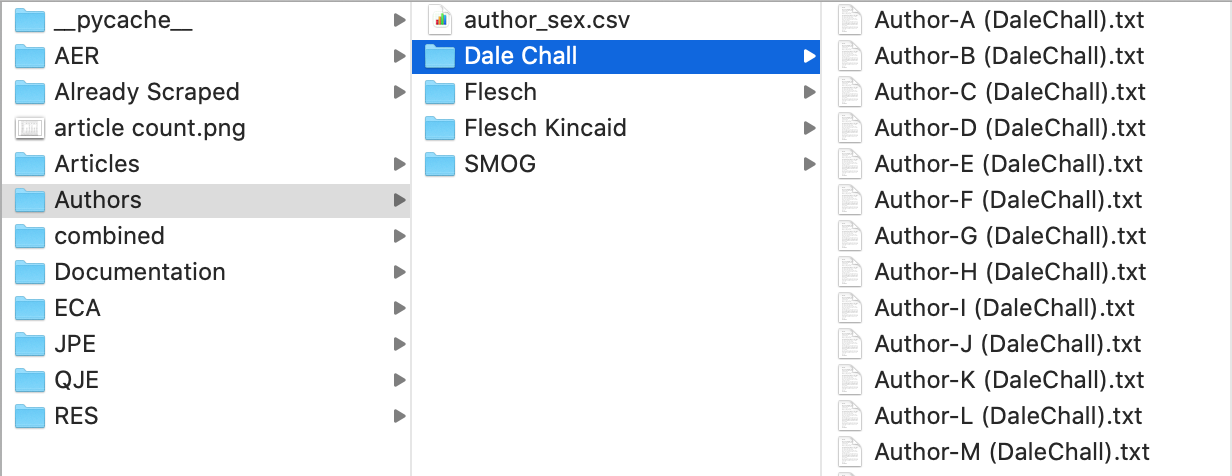
\includegraphics[width = 0.5 \textwidth]{IMG/author files.png}
    \caption{Where lists of authors and its information can be found}
    \label{fig:author_list}
\end{figure}

\subsubsection*{Author-Gender Detail}

The first-hand gender information that was directly extracted from the website is stored in 
\begin{center}
    \verb|Authors\author_sex.csv|
\end{center}

Directly using his data has several difficulties when matching it to the authors scraped. 
\begin{itemize}
    \item First name is abbreviated
    \item Middle names are neglected
    \item Special characters in name is interchanged with some English letters, such as ¨ø" to "o"
\end{itemize}

To overcome this, for each author, I created several equivalent "names". Transformation rules are coded in the first section of \verb|combined/transform_reg_data.ipynb|.
The final result is saved in 
\begin{center}
    \verb|combined/sex.csv|
\end{center}
This file matched all authors appearing in the \verb|all_combined.csv| and match its gender. 

Note that there are still several exceptions that are not captured by this rule, and is left as blank. Also, authors that only appears in REStud wasn't provided in Hengel's website\footnote{Her website only show results for AER, ECA, JPE, QJE for demonstrations.}. I excluded REStud atricles and save it in

\begin{center}
    \verb|combined/sex_noRes.csv|
\end{center}

The descriptive statistics are summarized in table \ref{tab:gender_miss}

\begin{table}[h]
    \centering
    \begin{tabular}{c c c c}
        \toprule \\
        Authors from & Male & Female & \# of Missing Gender \\
        \midrule \\
        Including REStud & 6241 & 1971 & 1173 \\
        Without REStud & 6101 & 1104 & 318 \\
        \bottomrule
    \end{tabular}
    \caption{Statistics of gender for journals including and excluding REStud}
    \label{tab:gender_miss}
\end{table}

I recommend doing further corrections in gender manually instead of looking for other patterns. 

\subsection{Regression-ready data}

I also came up with the program that turns the combined articles and the authors; information into a new data frame that is regression-ready. It is written in the second section\footnote{Note that the first section is the author-gender transformation part, described in the previous section.} of the file
\begin{center}
    \verb|combined/transform_reg_data.ipynb|
\end{center}
Named \emph{Get the data to be ready for regression}

The procedure is as following

\begin{enumerate}
    \item Load the combined data (From configuration)
    \item Load the gender information. It should be a \verb|json| format so that is can be turned into a \verb|dict| type. 
    \item Run all the function definitions and apply them.
\end{enumerate}

% I admit that the procedure is very messy and I want to apologies. It took me a while to read through what I did to explain. This is the final part that I am experiencing on but I am unable to spend much time on it. 




\bibliographystyle{econ}
\bibliography{ref.bib}

\end{document}

